% Created 2021-04-17 sab 19:00
% Intended LaTeX compiler: pdflatex
\documentclass[11pt]{article}
\usepackage[utf8]{inputenc}
\usepackage[T1]{fontenc}
\usepackage{graphicx}
\usepackage{grffile}
\usepackage{longtable}
\usepackage{wrapfig}
\usepackage{rotating}
\usepackage[normalem]{ulem}
\usepackage{amsmath}
\usepackage{textcomp}
\usepackage{amssymb}
\usepackage{capt-of}
\usepackage{hyperref}
\usepackage{float}
\usepackage[font={footnotesize,it}]{caption}
\usepackage[margin=0.7in, top=0.3in]{geometry} \pagenumbering{gobble} \usepackage{parskip}
\graphicspath{ {./Images/} }
\author{Alessandro Dangelo, 10524044 \\
Tancredi Covioli, 10498705}
\date{}
\title{Keep your distance Report}
\begin{document}

\maketitle

\section{Project proposal}
Design and implement a software prototype for a social distancing application using TinyOS and Node-Red and test it with Cooja. The application is meant to understand and alert you when two people (motes) are close to each other, and it is developed in three steps:

\begin{itemize}
  \item Each mote broadcasts its presence every 500ms with a message containing the ID number.
  \item When a mote is in the proximity area of another mote and receives 10 consecutive messages from that mote, it triggers an alarm. Such alarm contains the ID number of the two motes. It is shown in Cooja and forwarded to Node-Red via socket. 
  \item Upon the reception of the alert, Node-Red sends a notification through IFTTT to your mobile phone.
\end{itemize}

\section{Assumptions and implementation choices}
Some assumptions and implementation choices that have been made are:
\begin{itemize}
  \item \textbf{Distance range}: the distance range corresponds to the Transmission range of the mote. It is used the default value given by Cooja, which is an order of magnitude greater than a real social distancing application, but makes the management of the motes easier. Transmission ranges are equal for each mote.
  \item \textbf{Population size}: the population size is set to 10 (MAX\_NODES), since a greater number would have been not helpful for testing purposes. It can be increased by editing the header file.
  \item \textbf{Alarm message}: the alarm message is sent each time a mote receives 10 consecutive messages from the same corresponding mote, and it is sent again once 10 more messages are received. This approach was chosen to avoid a flood of incoming messages, expecially in crowded use cases in which social distancing may not be easily met.
  \item \textbf{Testing}: the system is tested with Cooja, since it gives the possibility to move motes in real time. Some tests have been made also in TOSSIM, but they have not been included in the documentation because they have been easily replicated in Cooja.
  \item \textbf{IFTTT notification}: the alarm message is displayed on the user's smartphone by a notification that appears in the notification menu. The Telegram message notification method was also tested, but it resulted in a more annoying experience.
\end{itemize}

\section{Mote's overwiew}
All motes are equal and they implement the same code: \newline
a mote has its own id, a personal counter and stores the status of the counters received from other motes around. \newline
\begin{wrapfigure}{r}{0.40\textwidth}
  \begin{center}
    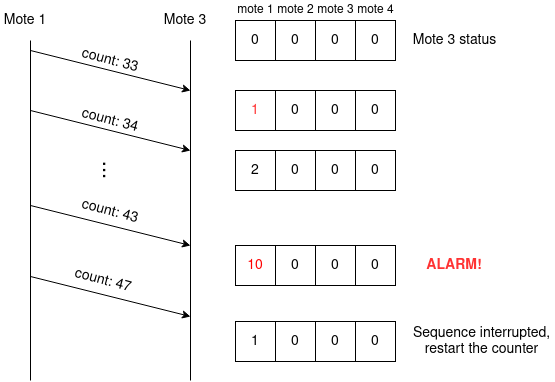
\includegraphics[width=0.40\textwidth]{status_update_diagram.png}
    \caption{evolution of the status of a mote}
  \end{center}
\end{wrapfigure}
When a mote starts its radio, the counter is set to 0. Once the message containing its own Id and the value of the counter is broadcasted, then the mote increments its counter. \newline
Upon reception of a new message, the mote updates its status by checking the sender ID, this way the corresponding value in the status is updated or reset, depending on the value stored and the new value received. \newline
If one of the counters in the status becomes a multiple of 10, then the alarm procedure is triggered and a message is sent. This message contains the IDs of the two motes (the one of the neighboring mote and its own) and the number of consecutive messages that either one received from the other. \newline
As soon as the two neighboring motes go away from each other, the alarm procedure is stopped.

\section{Node-Red flow overview}
The flow (shown in figure \ref{nodered}) begins with a TCP input node. This node is connected to a specific port, that corresponds to the port which a Cooja's mote is listening on. Each mote may potentially listening on a specific port, but in this case only one mote is set up this way for testing and debugging purposes. \newline
All incoming messages are filtered in the next step, this way only the alarm messages are forwarded. All these messages are then turned into sentences, without losing information. \newline
As last step, a IFTTT service is triggered by sending a URL request to the IFTTT API, containing the message.

\begin{figure}[H]
  \begin{minipage}{0.6\textwidth}
    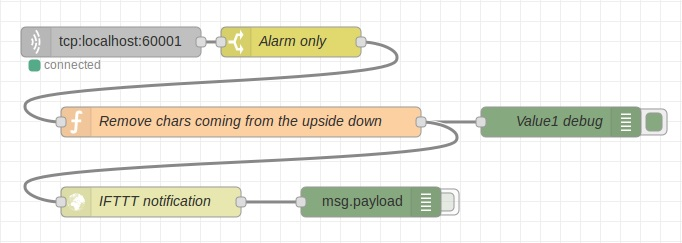
\includegraphics[height=108px]{Node-red-flow}
    \caption{Node-Red flow}
    \label{nodered}
  \end{minipage}
  \begin{minipage}{0.39\textwidth}
    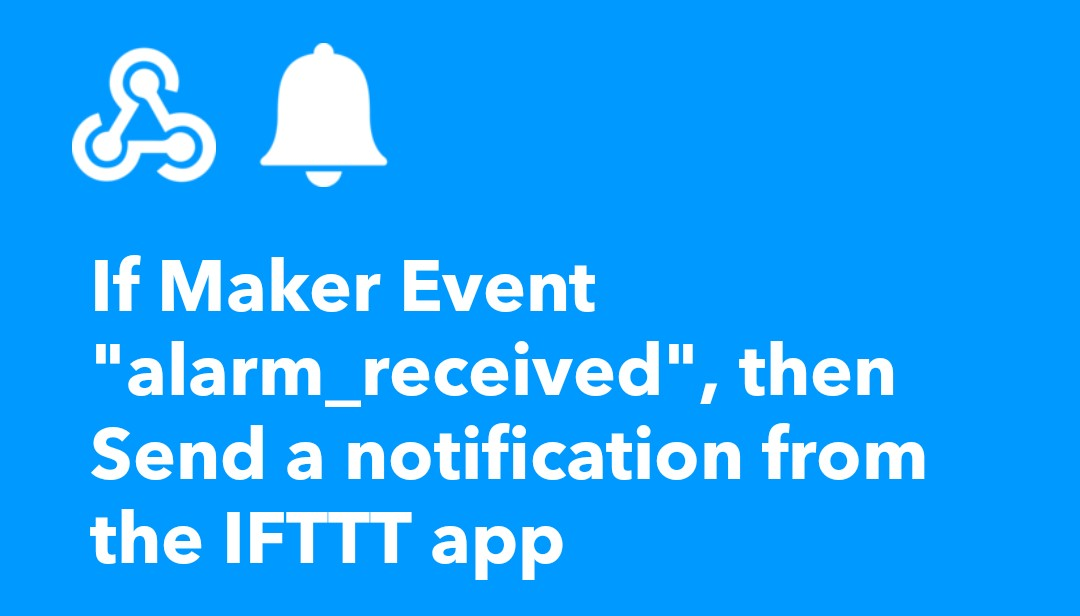
\includegraphics[height=108px]{ifttt-screenshot}
    \caption{IFTTT applet}
    \label{ifttt}
  \end{minipage}
\end{figure}

\section{IFTTT overview}
The IFTTT applet used works this way (as shown in figure \ref{ifttt}): \newline
IF the event "alarm\_received" is triggered \newline
THEN a notification is sent from the app.

\section{Simulation and testing}
The project was tested with several topologies; in this documentation a 10-mote simulation is described, since it seemed like a good middleground between stressing the system and discovering edge cases. \newline
During the simulation different scenarios were tested in sequence:
\begin{enumerate}
  \item All motes are far enough from each other in order not to violate the distantiation rule (\hyperref[distantiation]{figure on the left}).
  \item The motes form four groups with different number of members (\hyperref[small-groups]{center figure}).
  \item A group is dismantled and its members are assigned to different groups (\hyperref[crowded-groups]{figure on the right}).
\end{enumerate}

\begin{figure}[H]
  \centering
  \begin{minipage}{0.32\textwidth}
    \centering
    \frame{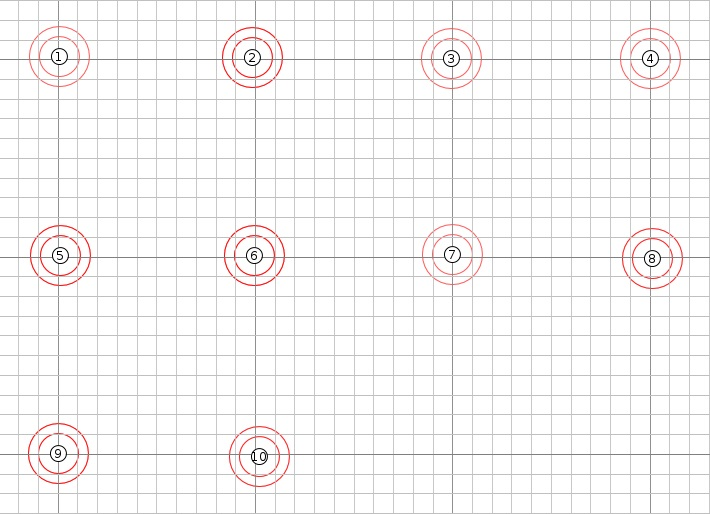
\includegraphics[height=118px]{Topology10-range-run}}
    \caption*{motes follow distantiation rule}
    \label{distantiation}
    
  \end{minipage}
  \begin{minipage}{0.32\textwidth}
    \centering
    \frame{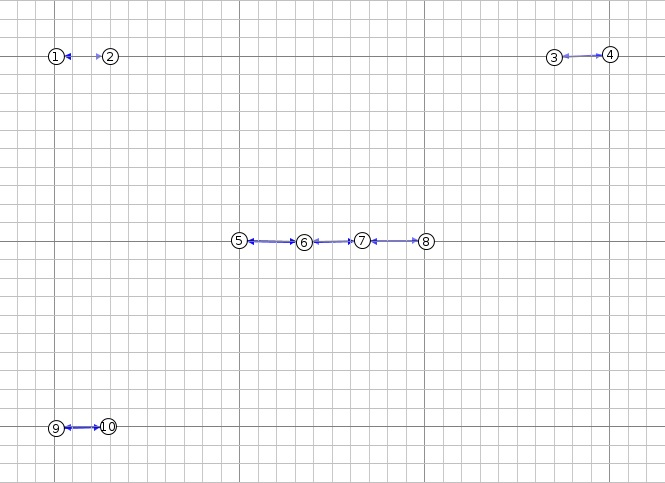
\includegraphics[height=118px]{Topology10-range-run-1_2-3_4-5_6_7_8-9_10}}
    \caption*{some small groups are created}
    \label{small-groups}
    
  \end{minipage}
  \begin{minipage}{0.32\textwidth}
    \centering
    \frame{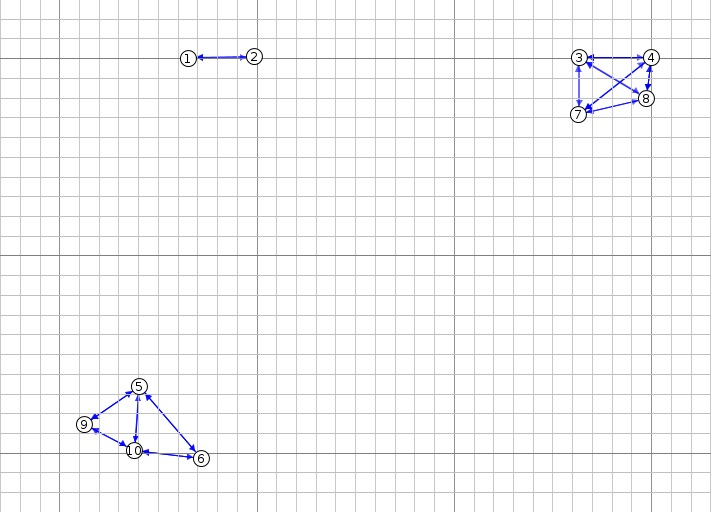
\includegraphics[height=118px]{Topology10-range-run-1_2-3_4_7_8-5_6_9_10}}
    \caption*{few crowded groups are created}
    \label{crowded-groups}
    
  \end{minipage}
\end{figure}

These scenarios were chosen in order to test the motes' behavior in a 1-to-1 situation and in a crowded environment that dynamically changes.

\subsection{Results}
Simulations had results in line with what it was expected, but two peculiar behaviors were encountered:

\begin{itemize}
  \item In a crowded environment, when many motes are near each other, the packets sent among the motes may collide and result in malformed messages being received. These messages are automatically discarded by the receiver, which will lose the sequence of incoming messages from its neighbours.
  \item In the remote case in which a mote is receiving packets while it is ready to transmit, the message reception is stopped and the transmission takes place. If this happens, the mote will lose the incoming message.
\end{itemize}

\begin{figure}[H]
  \centering
  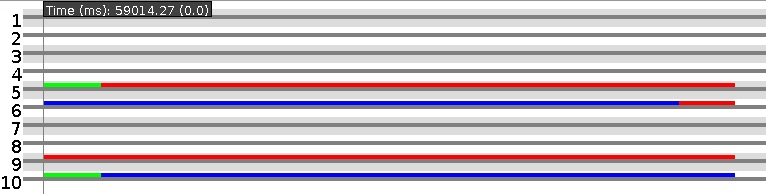
\includegraphics[width=0.8\textwidth]{10-motes-timeline.jpg}
  \caption{timeline of the two behaviors}
  \label{timeline}
\end{figure}

An example of the two behaviors can be noticed in the logs provided with this documentation (\texttt{log10motes}) at timestamp 59s. In figure \ref{timeline} we can notice that mote 6 starts the transmittion of a packet and a few milliseconds later mote 10 does the same. Mote 5, which is in range of both, receives corrupted data as soon as mote 10 starts its transmission because of the collision. \newline
At the same time, as mote 10 is receiving the packet from mote 6, its transmission timer fires and the reception is stopped. \newline
The result is that motes 5, 6, 10 miss a message and, in turn, reset their counter (as shown in figure \ref{log}).

\begin{figure}[H]
  \centering
  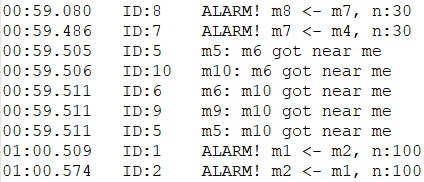
\includegraphics[width=0.40\textwidth]{LogTimeline.jpg}
  \caption{log section where the two behaviors take place}
  \label{log}  
\end{figure}

\end{document}
